\chapter{Contexte théorique et expérimental}
    \chapterprecishere{
        ``Potentielle citation sans aucun rapport avec le sujet"\par\raggedleft--- \textup{Personne inconnue}, contexte à déterminer
    }
    
    Le but de ce chapitre est de couvrir en quelques pages l'histoire des neutrinos, d'un point de vue théorique comme expérimental, de leur découverte jusqu'aux questions encore non résolues.
    
    \section{De la nécessité théorique à la place du neutrino dans la modèle standard}
    
	    \subsection{Brève histoire de la physique des particules}
	    
		    La physique des particules est une discipline mêlant électromagnétisme, mécanique quantique et relativité restreinte. Elle a pour objectif la description des interactions entres objets physiques à l'échelle la plus petite possible. La théorie de l'électromagnétisme de Maxwell, énoncée en 1864\cite{Maxwell1865}, est séparée de la genèse de la mécanique quantique et de la relativité restreinte par une quarantaine d'année seulement, ces deux dernières ayant vu le jour en 1900 et 1905 respectivement. 
		    
		    La première pierre de la mécanique quantique est la discrétisation des rayonnements d'un corps incandescent suggéré par Max Planck en 1900\cite{Planck1900}, bien que ce dernier ne la voyait alors que comme un artifice mathématique correspondant bien aux observations. Einstein, en 1905\cite{Einstein1905-quanta}, se basera sur le travail de Planck et proposera la notion de quantum de lumière appelé plus tard "photon" pour expliquer les résultats expérimentaux de l'effet photoélectrique observés en 1839 par Antoine Becquerel et Alexandre Edmond\cite{Becquerel1839}. Il publie sa théorie de la relativité restreinte\cite{Einstein1905-relat}, qui permet de se passer de la notion d'éther luminifère, ainsi que la très célèbre équation $E=mc^2$\cite{Einstein1905-emc2} la même année. La mécanique quantique continuera à s'étoffer jusqu'en 1930 avec les travaux de Bohr, de Broglie, Pauli, Schrödinger et Heisenberg pour aboutir à l'interprétation de Copenhague\cite{Heisenberg1949}. C'est à cette période que Pauli propose l'existence du neutrino\cite{Pauli1930}, nouvelle particule pas encore observée mais dont l'existence est nécessaire au maintien du principe de conservation de l'énergie (voir \autoref{sec::neutrino_origin}).
		    
		    Viennent ensuite les théories des interactions fondamentales et des champs de particules. Dirac propose son équation d'onde relativiste décrivant l'électron\cite{Dirac1928} (découvert en 1897 par Thomson\cite{Thomson1987}) en 1928, prédisant au passage la possibilité de l'existence de l'antimatière, le positron sera découvert en 1933 par Carl D. Anderson\cite{Anderson1933}. Fermi propose sa théorie expliquant la désintégration $\beta$ en 1934\cite{Fermi1934}, qui s'avérera être une approximation du modèle de Yukawa de 1935\cite{Yukawa1935} où les interaction se font via un échange de boson. Feynman, Schwinger et Tomonaga\cite{Tomonaga1946,Schwinger1948,Feynman1998} créent la théorie l'électrodynamique quantique entre 1946 et 1950, première forme du modèle standard que nous connaissons aujourd’hui. Cette théorie promeut le fait que les équations de Maxwell sont apparemment invariantes sous certaines transformation des champs électriques et magnétiques au rang de principe fondamental. Cette symétrie se traduit en mécanique quantique par l'invariance de la probabilité de présence d'une particule chargée sous un rephasage $U(1)$ pouvant dépendre de l'espace (transformation dite \textit{locale}). Imposer l'invariance sous cette transformation $U(1)$ local du lagrangien libre de cette même particule chargée abouti naturellement à l'apparition de termes d'interaction avec un champ de boson, qui n'est autre que le champ de photon, médiateur de l'interaction électromagnétique. Une très bonne introduction à ce concept peut se trouver dans "Geometry, particles and fields", de Bjorn Felsager \cite{felsager}.
		    
		    S'en suivent alors les découvertes de très nombreuses particules : de nombreux mésons, baryons et  hadrons, ainsi que le lepton $\nu$, ou muon, qui avait été découvert en 1937\cite{Street1937}. Les théories de Yang et Mills de 1954\cite{Yang1954} généralise l'invariance de jauge $U(1)$ de l'électrodynamique quantique et seront utilisées par Gell-Mann en 1961-1964\cite{Glashow1961,Gell-Mann1964} pour expliquer l'interaction forte tout en introduisant la notion de quarks comme composant fondamentaux du zoo de particules alors connues, et par Glashow, Salam et Weinberg en 1967\cite{Glashow1961a,Salam1964,Weinberg1967} pour unifier les interactions faible et électromagnétique en utilisant le mécanisme de brisure de symétrie postulée en 1964 par  Brout, Englert, Higgs, Hagen, Guralnik et Kibble\cite{Englert1964,Higgs1964,Higgs1964a,Kibble1967} prédisant l'existence du fameux boson de Higgs pour expliquer la génération des masses des particules alors connues. 
		    
		    Le neutrino électronique est découvert en 1956 par Cowan et Reine\cite{Cowan1956} auprès d'un réacteur nucléaire et le neutrino muonique sont observés en 1962\cite{Danby1962} au synchrotron AGS à Brookhaven, plus de 30 ans après leur proposition théorique. Le lepton $\tau$ est découvert en 1976\cite{Perl1975} avec l'anneau de collision SPEAR à SLAC, les bosons $Z^0$ et $W^{\pm}$ en 1983\cite{Arnison1983,Arnison1983a} avec l'expérience UA1 du CERN. Le dernier quark, le top, est découvert en 1995\cite{Collaboration1995} au Fermilab. Le neutrino tauique est découvert en 2000 par l'expérience DONUT\cite{Collaboration2000} et finalement le boson de Higgs est découvert en 2012 au LHC du CERN\cite{Collaboration2012}. Toutes les particules prédites et expliquées par le modèle standard de la physiques des particules, dont une représentation est montrée en \autoref{fig::standard_model}, ont alors été détectées. 
		    
		    Le puzzle du modèle standard est alors complet, et seul quelques phénomènes rares restent encore à observer. Tout ceci laisse cependant les physiciens sur leur faim : le modèle standard ne prédit pas tout (matière noire, gravitation...) et présente des particularités qui semble être des manifestations de phénomènes sous-jacent, notamment les grandes différences entre les masses des trois générations de particules (les trois colonnes de la \autoref{fig::standard_model}). Des théories au delà du modèle standard sont alors mises au point, comme la supersymétrie ou la théorie des cordes\cite{pdg2018}. Mais cette quête de nouvelle physique est pour le moment peu concluante : aucune particule supersymétrique n'a été détectée et les énergies actuelles ne permettent pas de tester bon nombre de nouvelles théories.
		    
		    L'avenir de la physique des particules était alors un peu sombre, jusqu'aux observations à la fin du XX$^{\text{ème}}$ et au début du XXI$^{\text{ème}}$ siècle du phénomène d'oscillation des neutrinos par les expériences Super-Kamiokande\cite{Fukuda1998} et SNO\cite{Aharmim2013}. Ces particules avaient joué un rôle secondaire dans le modèle standard jusque là. Le neutrino était certes nécessaire au maintien du principe de conservation de l'énergie, mais il ne prédisait rien en dehors de ça. Il avait cette particularité d'être de masse nulle, et de n'exister que dans un état de chiralité gauche, contrairement aux autres particules. Mais Super-Kamiokande et SNO ont observé qu'un neutrino initialement produit par un électron, donc dans un état de saveur électronique, peut produire à sa détection un neutrino d'une autre saveur, muonique ou tauique. Cette capacité qu'ont les neutrinos à changer de saveur est ce que l'on appelle "oscillation des neutrinos" et, comme nous allons le voir plus loin, elle requiers que les neutrinos aient une masse non nulle. Ce qui n'est pas prédit par le modèle standard de la physique des particules, et donc constitue de la nouvelle physique.
		    
		    Avant de rentrer dans les détails des oscillations des neutrinos, il convient de présenter un peu plus les caractéristiques de la particule la plus discrète du modèle standard.
		    		    
    
        \subsection{Le spectre d'énergie des électrons de désintégration \texorpdfstring{$\beta$}{b} : besoin d'une nouvelle particule}\label{sec::neutrino_origin}
        
	        La désintégration $\beta$ est la transformation spontanée d'un neutron neutron d'un noyau atomique en proton via l'émission d'un électron et d'un antineutrino électronique. L'énergie émise par une telle désintégration est égale, d'après la formule d'Einstein, à la différence des masses des noyaux avant et après désintégration multipliée par la vitesse de la lumière au carré : 
	        \begin{equation}
	        	Q = \left[m\left(^A_Z X\right)-m\left(^A_{Z+1} X\right)\right]c^2
	        \end{equation}
	        Pour un type de noyau $\left(^A_Z X\right)$, cette énergie est constante. La conservation de l'énergie nous dit alors que
	        \begin{equation}
	        	E_{initial} = E_{final} +E_{e^-}+E_{\overline{\nu}_e} = E_{final}+Q
	        \end{equation}
	        où $E_{initial}$ est l'énergie totale du noyau avant désintégration, $E_{final}$ est son énergie après désintégration et $E_{e^-}$ et $E_{\overline{\nu}_e}$ sont les énergies de l'électron et de l'antineutrino. On a donc $E_{e^-}+E_{\overline{\nu}_e} = Q$.
	        
	         Au moment de la proposition de l'existence du neutrino par Wolfgang Pauli en 1930\cite{Pauli1930}, seul l'électron et le noyau après désintégration étaient détectables, aussi le terme d'énergie $E_{\overline{\nu}_e}$ était absent de l'équation précédente. Dans ce cas là, pour une source radioactive donnée, puisque $Q$ est constante, le spectre en énergie de l'électron aurait due être très piqué atour de $Q$. Or ce n'est pas le cas : ce spectre est continue (voir \autoref{fig::beta_spectrum}) entre 0 et $Q$. En revanche, rajouter à la réaction une particule jusque là invisible correspond parfaitement à ce spectre, pourvu que la masse de cette particule soit très petite devant $Q$. En effet, si l'antineutrino (et donc le neutrino) avait une masse conséquente, le spectre de l'énergie de l'électron ne pourrait pas atteindre la valeur de $Q$, puisqu'un partie irréductible de $Q$ va dans la masse du neutrino. C'est d'ailleurs un mesurant avec une très grande précision le spectre de l'énergie des électrons issues de la désintégration du tritium que l'expérience KATRIN\cite{Kleesiek2018} pourra déterminer la masse effective du neutrino électronique avec une précision de \SI{0.2}{\electronvolt\per c\squared}.
    
        \subsection{Premières observations directes du neutrino}
        
	        Entre les années 30 et 50, la détection du neutrino semblait hors de porté. Il était connu que la probabilité d'interaction de cette particule étant très faible, et seule un source très intense de neutrinos pouvait permettre leur observation. Le développement de l'énergie nucléaire dans les années 50 a fourni cette source : les réactions de fission sont accompagnée de l'émission d'antineutrinos électroniques en très grande quantité.
	        
	        Entre 1952 et 1953, Frederick Reines et Clyde Cowan construisent un détecteur dont le matériau de réaction est simplement de l'eau. Un antineutrino incident, si il rencontre un proton, fera une réaction $\beta$ inverse produisant un neutron et un positron, se dernier d'annihilant rapidement avec un électron pour donner deux photons. Le signal attendu est alors la détection de deux photon suivi par l'interaction d'un neutron avec l'eau caractérisé par l'émission d'un troisième photon, après absorption du neutron par un noyau de chlorure de cadmium, un bon absorbeur de neutron que Reines et Cowan ont dissous dans l'eau. La détection des photons s'effectuaient dans une couche de scintillateur liquide munie de tubes photomultiplicateurs entourant les deux cuves de détection. Le volume d'eau totale était de $\SI{200}{\liter}$ où étaient dissous $\SI{40}{\kilogram}$ de chlorure de cadmium. Le flux de d'antineutrinos attendu du réacteur était de $\SI{5e13}{\overline{\nu}_e\second^{-1}\centi\meter^{-2}}$\cite{ref_needed}.
	    
		    La première tentative de détection du neutrino fut faite proche du réacteur nucléaire de Hanford dans l'état de Washington, sans donner de résultats concluant. La seconde tentative, proche du réacteur de Savannah River en Caroline du Sud, détecta un signal de \SI{2.88}{\text{counts}\per\hour}\cite{Cowan1956} pour 1371 heures de prises de données, 20 fois supérieur au bruit de fond attendu, démontrant finalement l'existence d'une particule légère, et particulièrement peu réactive, dans la réaction $\beta$. La section efficace mesurée de  \SI{6.3e-44}{\centi\meter\squared} était compatible avec la valeur tirée des mesures de désintégration du neutron de Robson\cite{Robson1951}, de \SI{6e-44}{\centi\meter\squared}.
		    
		    Aujourd'hui, les expériences cherchant à détecter des neutrinos sont conçues de manière semblable à l'expérience de Reines et Cowan : un volume aussi grand et aussi dense que possible afin d'offrir un maximum de cibles sur lesquels les neutrinos  peuvent interagir, une source intense et un temps d'exposition long. La réduction du bruit de fond est essentielle dans une telle expérience : lors de leur seconde tentative, Reines et Cowan ont placé leur détecteur sous terre afin de mieux se protéger des rayons cosmiques. Cette technique est encore largement employée aujourd'hui dans presque toutes les expériences détectant des neutrinos.
		    
		    L'eau est encore utilisée, par exemple dans l'expérience Super-Kamiokande\cite{Fukuda1998}, mais des matériaux solides ont également permit la détection de neutrinos comme dans les expériences NO$\nu$A\cite{ref_needed} et OPERA\cite{opera}. Une des techniques les plus récentes utilise comme cible des gaz nobles liquéfiés, bien plus dense que l'eau, notamment l'argon dans l'expérience prototype ICARUS\cite{Amerio2004} et la future expérience \gls{dune}\cite{Acciari2016a}. 
		    
		    Les réacteurs nucléaires sont encore beaucoup utilisés dans les expériences de neutrinos, par exemple par Double Chooz\cite{ref_needed}, Daya Bay\cite{ref_needed} et la future JUNO\cite{ref_needed}. Des faisceau de neutrinos créés artificiellement ont également vu le jour dans les années 60, servant de sources à des expériences comme T2K\cite{ref_needed} ou \gls{dune}\cite{Strait2016}. Des sources naturelles existent aussi : le soleil fourni un important flux de neutrinos, étudié par des expériences comme SNO\cite{ref_needed}. Ces derniers, avec les neutrinos produits par des rayons cosmiques dans l'atmosphère et détectés par Super-Kamiokande\cite{Fukuda1998} ont permis de mettre en évidence le phénomène d'oscillation des neutrinos et ont reçu le prix Nobel en 2015. Enfin, les neutrinos issues de supernovae peuvent également être détectés, pourvu qu'une supernovae explose durant une prise de donnée d'une expérience. C'est arrivé une seule fois en 1987, où 20 événements neutrinos ont été détectés par les détecteur IMB et Kamikande II\cite{Hirata1987}.
		    
		\subsection{Parité et hélicité : le neutrino vote à gauche}
		
			Un transformation de parité consiste à prendre un système ou processus physique  et à le regarder dans un miroir. Autrement dit, remplacer toutes les coordonnées d'espace par leur opposées : $\Vec{r}\to-\Vec{r}$.
			
			Si la parité laisse le système ou processus inchangé, ce dernier est dit pair. Si au contraire il devient son opposé, il est dit impaire. L'exemple classique d'objet physique impaire est l'impulsion : $\Vec{p}(-\Vec{r}) = m(-\dot{\Vec{r}}) = -\Vec{p}(\Vec{r})$. À l'inverse, un objet pair est le moment cinétique : $\Vec{L}(-\Vec{r}) = -\Vec{r}\times -\Vec{p} = \Vec{L}(\Vec{r})$. L'extension à la mécanique quantique consiste à dire qu'un état est pair(impair) si il est état propre de l'opérateur de transformation de parité $\hat{P}$ avec une valeur propre de $+1(-1)$.
			
			En 1954, Chinowsky et Steinberger\cite{ref_needed} montrent que le pion $\pi$ est toujours impair. La même année, deux particules de même masse et de même temps de vie, mais avec des états de désintégration avec des parités différentes sont découvertes\cite{ref_needed} : le $\theta^+$ se désintègre en $\pi^+ + \pi^0$, qui ont à eux deux une parité de $-1\times-1=1$, tandis que le le $\tau^+$\footnote{Cette particule n'a rien à voir avec le lepton $\tau$.} se désintègre en $\pi^+ + \pi^+ + \pi^-$, qui ont à eux trois une parité de $-1\times-1\times-1=-1$. Le fait que ces deux particules soit si semblable en dehors de la parité de leurs états finaux amène les scientifiques à envisager qu'il s'agit en fait d'une seule particule\footnote{Il s'agit en réalité du kaon $K^+$.} et que la transformation de parité n'est pas une symétrie de la nature.
			
			En 1956, Tsung Dao Lee et Chen Ning Yang se rendent compte que, bien que bon nombre d'expériences montrent que l'interaction forte et électromagnétique sont symétriques par transformation de parité, aucune n'a étudié la question pour l'interaction faible. Ils proposent alors plusieurs méthodes expérimentales dont une, qui consiste à étudier la distribution spatiale des électrons émis par des noyaux radioactifs $\beta$ avec des spins alignés, est mise en œuvre entre 1956 et 1957 par Chieng-Shiung Wu. La \autoref{fig::wu} schématise le signal recherché : l'image miroir d'un noyau émettant un électron dans la même direction que son spin est le même noyau émettant cet électron dans la direction opposé au spin, puisque le spin est invariant par transformation de parité. Le processus miroir est donc différent du processus initial et donc, pour que la désintégration $\beta$ soit symétrique par rapport à la transformation de parité, il faut qu'un ensemble de noyaux radioactifs dont les spins sont aligné émettent autant d'électrons dans le direction de leur spin que dans la direction opposée. Or, l'expérience montre que ce n'est pas le cas : l'électron est en écrasante majorité émis dans la direction opposée au spin\cite{ref_needed}.
			
			En plus de résoudre de problème des particules $\theta^+$ et $tau^+$, ce résultat apporte une information sur le neutrino : si l'électron est toujours émis dans la direction opposé au spin du noyau, alors l'antineutrino, émis dans la direction du spin, est d'hélicité droite. L'hélicité est la projection du spin sur l'impulsion, une particule est dite "d'hélicité droite" si spin et impulsion sont dans la même direction et d'hélicité "gauche" si ils sont dans des directions opposées. L'hélicité du neutrino est mesurée précisément en 1957 par Goldhaber\cite{ref_needed}, et révèle que ce dernier est d'hélicité gauche. Le neutrino est alors la seule particule élémentaire connues à ne pouvoir exister que dans un état d'hélicité. Cette particularité joue un rôle important sur l'origine de la masse des neutrinos, comme nous allons le montrer plus loins.
    
        \subsection{Les 3 familles de neutrinos}
        
	        Le muon, découvert en 1937 par Street et Stevenson\cite{Street1937}, n'a a priori comme différence avec l'électron que sa masse. Ce dernier étant (théoriquement, à l'époque) produit avec un neutrino dans les désintégrations $\beta$, il paraissait plausible que le muon puisse également être lié au neutrino d'une manière ou d'une autre.  Le spectre en énergie de l'électron produit par la désintégration du muon, mesuré par Leighton, Anderson et Seriff en 1949\cite{Leighton1949}, est continue. Un raisonnement identique à celui de Pauli de 1930 montre que le muon doit se désintégrer en trois particules : un électron et deux neutrinos. Il fallut cependant attendre 1962 et les expériences de faisceau de neutrinos de Lederman, Steinberger et Schwartz\cite{Danby1962} pour détecter le neutrino muonique et définitivement montrer qu'il était différent du neutrino électronique : les neutrinos du faisceau, produits par la désintégration de muons, ne créaient que des muons dans le détecteur et aucun électron.
	        
	        La découverte du troisième lepton, le $\tau$, en 1975 par Perl\cite{Perl1975} n'a pas tardé à être suivi par la prédiction d'un troisième neutrino associé, le neutrino tauique. Ce dernier fut détecté en 2000 par l'expérience DONUT\cite{Collaboration2000}. Un faisceau de neutrino issu du fermilab, contenant toutes les saveurs possibles de neutrino interagit avec un détecteur capable de d'identifier les produits de réactions, qui a identifié 4 événements neutrinos ayant créé un $\tau$.
	        
	        A ce moment là, les trois familles de quarks up--down, strange--charmed et top--bottom et les trois familles de leptons, l'électron et son neutrino, le muon et son neutrino et le tau et son neutrino, avaient été détectées. L'expérience ALEPH, au LEP, en étudiant la désintégration du boson $Z$, un des vecteurs de l'interaction faible, avait montré en 1989 qu'il ne pouvait pas exister plus de 3 saveurs de neutrinos pouvant interagir avec le $Z$\cite{DeCamp1989}. Tous les neutrinos détectables avaient alors été détectés.
        
        \subsection{Dirac vs Majorana}\label{sec::dirac_majorana}
        
	        
    
    \section{Le paradigme des oscillations des neutrinos}
    
        \subsection{Genèse de la théorie}
        
            On désigne habituellement un neutrino par sa saveur : neutrinos muonique ($\nu_{\mu}$), électronique ($\nu_e$) ou tauique($\nu_{\tau}$). Un neutrino est dans l'un de ces 3 "états de saveur" si il est produit par le lepton qui y correspond, ou si il produit ce lepton en interagissant avec son environnement. Rien, à priori, n'oblige le lepton qui créé le neutrino à être de même saveur que le lepton créé par le neutrino après interaction. Le premier à avoir soulevé ceci est Bruno Pontecorvo, même si il ne l'a pas fait en ces termes. En effet, au moment de la publication de ses deux premiers articles\cite{Pontecorvo:1957cp,Pontecorvo:1957qd} sur le sujet à la fin des années 60, il n'était pas connu qu'il y avait plusieurs saveurs de neutrino. B.~Pontecorvo parlait de possible transition entre neutrino et antineutrino du fait que le neutrino soit neutre, inspiré par les travaux de Gell-Mann et Païs\cite{Gell-Mann1955} sur la conversion du $\overline{K^0}$ en  $K^0$. Dans son article suivant en 1968\cite{Pontecorvo1968}, tout en gardant la possibilité de conversion des neutrinos vers les antineutrinos, il introduit la possibilité d'une conversion du neutrino électronique vers le neutrino muonique, découvert en 1962\cite{Danby1962}. Il prédira également deux résultats importants :
            \begin{itemize}
                \item Si les masses des neutrinos ne sont pas nulles et que la charge leptonique n'est pas être conservée, les neutrinos peuvent changer de saveur
                \item Un déficit de neutrinos en provenance du soleil d'un facteur 2 environ par rapport au prédiction du modèle solaire standard est attendu dans ce cas
            \end{itemize}
            La première prédiction implique de la physique au delà du modèle standard de la physique des particules, puisque ce dernier suppose que les masses des neutrinos sont nulles. Mais ceci n'est pas imposé par la théorie : il a été expérimentalement observé dans toutes les expériences à ce jour que les neutrinos se comportent, si ce n'est comme des particules de masses nulles, comme des particules de masse suffisamment faible pour être négligée. 
            La seconde prédiction fut vérifiée en 1970 par la Brookhaven Solar Neutrino Experiment\cite{Bahcall1976}, qui trouva un déficit compris entre 2 et 3. Il ne s'agissait alors pas encore d'une preuve, d'autre théorie pouvant expliquer ce phénomène, mais c'était un indice qui a incité les chercheurs à creuser la question.
            
            Le changement de saveur $\nu_e\rightleftharpoons\nu_{\mu}$ avait été envisagé également entre 1962 et 1963 par deux groupes de physiciens, Katayama, Matumoto, Tanaka et Yamada\cite{Nakagawa1963} puis que Ziro Maki, Masami Nakagawa and Shoichi Sakata\cite{Maki1962}. Ces quatre derniers donneront leurs noms, avec Pontecorvo, à la célèbre matrice \gls{pmns} décrite plus loin. Leur point de départ était différent de celui de Pontecorvo, puisqu'ils visaient à créer une théorie unifiant les leptons et les hadrons. Ils sont également arrivé à la conclusion qu'une oscillation des neutrinos implique que ces derniers doivent avoir des masses non nulles.
            
            En 2015, Arthur~B.~McDonald et Takaaki Kajita ont reçu le prix Nobel de physique pour "pour la découverte des oscillations des neutrinos, qui montre que les neutrinos ont une masse". Les deux expériences ayant fait cette découverte sont SNO\cite{Aharmim2013} et Super-Kamiokande\cite{Fukuda1998}.
            
            \begin{figure}[htbp]
                \begin{subfigure}[t]{0.56\textwidth}
                    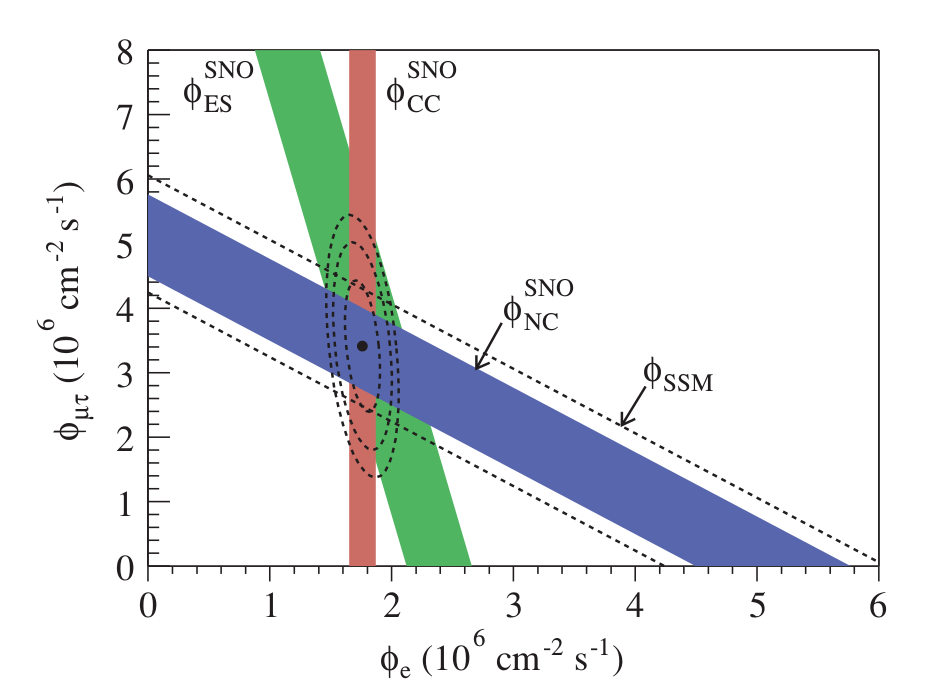
\includegraphics[width=\textwidth]{Chapitre_1/pictures/SNO_plot.png}
                    \caption{Mesure des composantes $\nu_{\mu}$ et $\nu_{\tau}$ du flux de neutrino solaire contre la composante $\nu_e$\cite{Aharmim2013}. Le flux total mesuré ($\phi_{NC}^{SNO}$) est consistant avec le flux total prédit ($\phi_{SSM}$). La composante électronique du flux ($\phi_{CC}^{SNO}$), qui devrait constituer $100\%$ du flux sans oscillations, n'en représente que $35\%$, ce qui indique un changement de saveur.}
                    \label{fig::SNO_plot}
                \end{subfigure}
                \hfill 
                \begin{subfigure}[t]{0.4\textwidth}
                    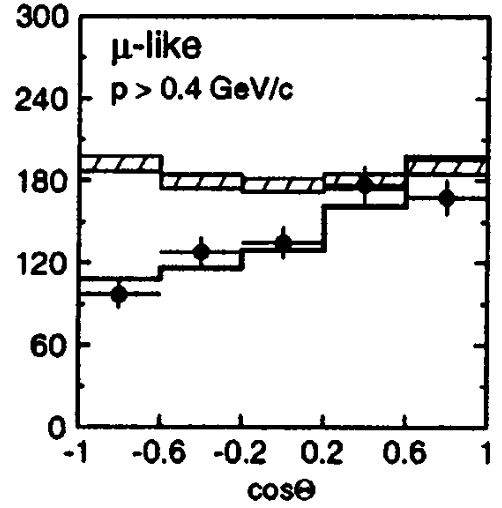
\includegraphics[width=\textwidth]{Chapitre_1/pictures/superK_plot.png}
                    \caption{Nombre de neutrinos muoniques mesurés par Super-Kamiokande (traits pleins) et prédit par le Monte Carlo (traits pointillés) pour un an et demi de prise de donnée contre l'angle zénithal avec lequel le neutrino arrivait\cite{Fukuda1998}. Un cosinus négative correspond à un neutrino ayant traversé la Terre. La différence entre observation et prédiction à grand angle indique une disparition des neutrinos muonique.}
                    \label{fig::superK_plot}
                \end{subfigure}
            \end{figure}
            
            SNO détectait les neutrinos solaires, par interaction par courant chargé (CC) et par courant neutre (CN), permettant d'avoir accès à la fois au flux de neutrinos électroniques (CN et CC) et au flux de neutrios muoniques et tauiques (CN). Comme le montre la \autoref{fig::SNO_plot}, la somme des trois flux correspond bien au flux total prédit par le modèle solaire standard alors que le flux de neutrinos électronique est inférieur aux prédiction, montrant qu'une partie du flux change de saveur mais que le flux total est conservé.
            
            Super-Kamiokande détectait des neutrinos issues des interactions de rayons cosmiques avec l'atmosphère. Il pouvait ainsi comparer les flux des neutrinos pour différents angles zénithaux, correspondant à des créations du neutrino allant de juste au dessus du détecteur (angle nul) à l'autre bout du globe (angle de $\pi$). Comme nous allons le montrer plus loin, la probabilité qu'a un neutrino de changer de saveur dépend de la distance parcoure (équation \eqref{eq::proba_oscillation}). Une dépendance du flux en l'angle zénithal a donc indiqué un phénomène de changement de saveur. La figure \autoref{fig::superK_plot} montre cette dépendance pour des événements de neutrinos muoniques.
    
        \subsection{Pourquoi "Oscillations"?}\label{sec::oscillations}
            La base de la théorie de l'oscillation des neutrinos est de dire que les états $\nu_e$ $\nu_{\mu}$ et $\nu_{\tau}$ sont -- par définition -- des états propres du lagrangien d'interaction, mais pas forcément des états propres de l'hamiltonien, appelés également états propres de masse. Autrement dit, il n'est pas forcément possible de décrire la propagation dans l'espace temps d'un état de saveur. Partons du principe que les états de saveurs des neutrinos ne sont en effet \textit{pas} des états propres de masse et regardons les conséquences. 
            
            \subsubsection{Conventions de notation}
            \begin{itemize}
                \item $\hbar = c = 1$ (système d'unité naturelle)
                \item Nous supposerons que toutes les fonctions d'ondes décrites sont suffisamment loin de leur source pour être considérées comme des ondes planes. Les expériences de neutrinos vérifient généralement facilement cette conditions.
                \item $\nu_e$ $\nu_{\mu}$ et $\nu_{\tau}$ sont les états propres de saveur. Un neutrino est dans un de ces états au moment de sa création et au moment de sa destruction.
                \item $\nu_{\alpha,\beta...}$ désigne un des trois états propres de saveur.
                \item $\l_{\alpha,\beta...}$ désigne un des trois leptons chargés $e$, $\mu$ ou $\tau$.
                \item $U_{\alpha i}$ est un élément de la matrice $U$ permettant de passe de la base des états propres de saveur à la base des états propres de masse.
                \item $\nu_{i}$ avec $i$ un entier non nul désigne un état propre de masse, qui vérifie l'équation
                \begin{equation}
                    \ket{\nu_i(t)} = e^{-i(E_i\cdot t - p_i\cdot x)}\ket{\nu_i(0)}.
                \end{equation}
            \end{itemize}
            
            \subsubsection{Superposition des états de masse}
            Les états de saveurs, si ils ne sont pas des états de masses, sont une superposition linéaire de ces états. On peut donc écrire
            \begin{eqnarray}
            \ket{\nu_{\alpha}} = \sum_i U_{\alpha i}^*\ket{\nu_i} \label{eq::alphatoi} \\
            \ket{\nu_i} = \sum_{\alpha} U_{\alpha i}\ket{\nu_{\alpha}}.
            \end{eqnarray}
            
            L'état d'un neutrino initialement créé dans une saveur $\alpha$ est alors :
            \begin{equation}
            	\ket{\nu(t=0)} = \ket{\nu_{\alpha}} = \sum_i U_{\alpha i}^*\ket{\nu_i(t=0)}
            \end{equation}
            Son état à un temps $t > 0$ est alors :
            \begin{equation}
	            \begin{split}
	            	\ket{\nu(t)} &=\sum_{i} U_{\alpha i}^*\ket{\nu_i(t)} = \sum_{i} U_{\alpha i}^* e^{-i(E_i\cdot t - p_i\cdot x)}\ket{\nu_i(0)} = \sum_{i} U_{\alpha i}^* e^{-i(E_i\cdot t - p_i\cdot x)}\sum_{\beta}U_{\beta i}\ket{\nu_{\beta}}\\ & = \sum_{i,\beta} U_{\alpha i}^*U_{\beta i} e^{-i(E_i\cdot t - p_i\cdot x)}\ket{\nu_{\beta}}
            	\end{split}
            \end{equation}
            
            Plusieurs points méritent d'être soulignés ici :
            \begin{itemize}
                \item Un état de saveur $\alpha$ ne peut interagir qu'avec un lepton de même saveur. Les états de saveur doivent donc être orthogonaux
                \item Il a été montré expérimentalement qu'il ne peut exister que trois états de saveurs actives (i.e qui se couplent au boson $Z$)\cite{pdg2018}.
                \item Il faut donc au moins trois états de masse. Si il en existe plus que trois, cela implique qu'il existe d'autres états de saveur qui ne se couplent pas avec le boson $Z$. De tels états, dit "stériles" sont de potentiels candidats pour la matière noire.
                \item La matrice $U$ étant une matrice de changement de base, elle doit être unitaire :
                \begin{equation*}
                    \delta_{\alpha\beta} = \braket{\nu_{\alpha}}{\nu_{\beta}} = \braket{\sum_i U_{\alpha i}\nu_i}{\sum_j U_{\beta j}^*\nu_j} = \sum_{i,j} U_{\alpha i}U_{\beta j}^* \braket{\nu_i}{\nu_j} = \sum_{i,j} U_{\alpha i}U_{\beta j}^*.
                \end{equation*}
            \end{itemize}
            Comme nous ne pouvons détecter que les trois états de saveur $\nu_e$ $\nu_{\mu}$ et $\nu_{\tau}$, il convient de travailler avec un matrice $3\times3$. La combinaison des mesures actuelles et futures des éléments de cette matrice\cite{Qian2013} permettra de tester si cette matrice est unitaire. Si ce n'est pas le cas, cela prouvera l'existence des neutrinos stériles car alors la matrice $3\times3$ ne sera qu'une sous-matrice d'une matrice plus grande qui, elle, doit être unitaire.
            
            Avant de détailler cette matrice $U$, intéressons nous à la question suivante : \\
            \subsubsection{Quelle est la probabilité de passer d'une saveur $\beta$ vers une saveur $\alpha$?}
            En notant $\ket{\nu(t)}$ l'état de masse dans lequel se trouve un neutrino à un instant $t$ , cette probabilité est donnée par la projection de l'état de saveur $\beta$ sur cet état :
            \begin{equation}
                P(\nu_{\alpha}\to\nu_{\beta})=\bigg|\braket{\nu_{\beta}}{\nu(t)}\bigg|^2.
            \end{equation}
            En utilisant l'équation \eqref{eq::alphatoi} on montre que
            \begin{equation}
                \braket{\nu_{\beta}}{\nu(t)} = \sum_i U_{\alpha i}^*U_{\beta i} e^{-i(E_i\cdot t - p_i\cdot x)}.
            \end{equation}
            Ici aussi plusieurs choses sont à noter : 
            \begin{itemize}
                \item $t$ correspond au temps écouler entre la création et la destruction du neutrino dans le référentiel du détecteur. Ce temps n'est généralement pas mesurable, étant donné que les sources de neutrinos en émettent continument
                \item $x$ correspond à la distance parcourue par le neutrino. Nous la noterons $L$ dans la suite du texte et l'appellerons \textit{ligne de base}. Elle est mesurable puisque c'est la distance entre la source et le détecteur.
                \item Si le modèle standard considère les neutrinos comme non massifs, c'est que leur masse est trop petite pour jouer un rôles dans les mesures d'énergie et d'impulsion. Il est donc correcte d'approximer $p_i \simeq E_i - \frac{m_i^2}{2E_i}$
            \end{itemize}
            Dans une expérience détectant des neutrinos, la probabilité sera moyennée sur le temps $t$, inconnu. Supposons que la source des neutrinos ait deux composantes d'énergies différentes $E_1$ et $E_2$, contribuant de manière cohérente au signal observé dans le détecteur. Au bout du temps $t$, chaque composante aura pris un facteur de phase $e^{-iE_jt}$. Les interférences entre les deux composantes feront alors entrer en jeu un facteur de phase $e^{-i(E_1-E_2)t}$. Moyenné sur $t$, ce facteur disparaît, sauf si $E_1 = E_2$. Les seules composantes contribuant de manière cohérente au signal ont donc une même énergie $E$. Ce point est détaillé ici dans les articles de Stodolsky\cite{Stodolsky1998}, Lipkin\cite{Lipkin2005} et Kayser\cite{Kayser2005}. On se retrouve donc avec l'équation suivante : 
            \begin{equation*}
                P(\nu_{\alpha}\to\nu_{\beta}) = \bigg|\sum_i U_{\alpha i}^*U_{\beta i} e^{-im_i^2\frac{L}{2E}}\bigg|^2.
            \end{equation*}
            Cette expression peut se mettre sous forme sinusoïdale\cite{Mondal2015} :
            \begin{equation}\label{eq::proba_oscillation}
                \begin{split}
                    P(\nu_{\alpha}\to\nu_{\beta}) = \delta_{\alpha\beta} & - 4\sum_{i>j}\Re(U_{\alpha i}U_{\beta i}^*U_{\alpha j}^*U_{\beta j})\sin^2\left(\Delta m_{ij}^2\frac{L}{4E}\right) \\
                    & +2\sum_{i>j}\Im(U_{\alpha i}U_{\beta i}^*U_{\alpha j}^*U_{\beta j})\sin\left(\Delta m_{ij}^2\frac{L}{2E}\right)
                \end{split}
            \end{equation}
            où $\Delta m_{ij}^2 = m_i^2-m_j^2$. Il peut être utile de définir une longueur d'oscillation $l_{osc} = 4\pi E/\Delta m_{ij}^2$ si l'on souhaite étudier les oscillations en fonction de la ligne de base $L$ pour des énergies fixées, réécrivant alors les termes en $\sin$ et $\sin^2$ :
            \begin{eqnarray}
                \sin^2\left(\Delta m_{ij}^2\frac{L}{4E}\right) = &  \sin^2\left(\pi\frac{L}{l_{osc}}\right) \\
                \sin\left(\Delta m_{ij}^2\frac{L}{2E}\right) = & \sin\left(2\pi\frac{L}{l_{osc}}\right).
            \end{eqnarray}
            
            On peut noter trois choses:
            \begin{itemize}
                \item Le terme "oscillation" est ici évident : la probabilité qu'a un neutrinos de changer de saveur est une fonction sinusoïdale du ration $\frac{L}{E}$. 
                \item La masse d'un neutrino ne sera pas accessible par mesure de probabilité d'oscillation : seule une différence de masse carré est accessible. On ne peut donc pas, avec les oscillations des neutrinos, déterminer les valeurs des masses des neutrinos. On peut juste dire que deux sont non nulles.
                \item Il suffit de mesurer deux $\Delta m_{ij}^2$ pour pouvoir calculer le dernier
                \item La somme $\sum_{\beta\in\{e,\mu,\nu\}}P(\nu_{\alpha}\to\nu_{\beta})$ doit être égal à 1 de par l'unitarité de $U$. Un neutrino ne disparaît pas, il change juste de saveur. Mais si une de ces saveurs n'est pas observable parce que stérile, alors le flux total observable s'en verra diminué. Les résultats de SNO montrés en \autoref{fig::SNO_plot} tendent à montrer que la probabilité d'osciller vers un tel état est faible, au moins aux valeurs de $L/E$ correspondant aux neutrinos solaires.
                \item Les expériences mesurant les oscillations des neutrinos sont souvent caractérisés par leur \textit{ligne de base} $L$, qui est la distance entre le détecteur et la source et correspond au $L$ des équations précédentes.
            \end{itemize}
            
            On peut immédiatement calculer la même probabilité pour les antineutrinos, en supposant que la symétrie CPT n'est pas violée : 
            \begin{equation}
                P(\overline{\nu}_{\alpha}\to\overline{\nu}_{\beta}) = P(\nu_{\beta}\to\nu_{\alpha}).
            \end{equation}
            La partie réelle de l'équation \eqref{eq::proba_oscillation} restera inchangée, tandis que la partie imaginaire deviendra négative. On aura donc :
            \begin{equation}
                \begin{split}
                    P(\overline{\nu}_{\alpha}\to\overline{\nu}_{\beta}) = \delta_{\alpha\beta} & - 4\sum_{i>j}\Re(U_{\alpha i}U_{\beta i}^*U_{\alpha j}^*U_{\beta j})\sin^2\left(\Delta m_{ij}^2\frac{L}{4E}\right) \\
                    & -2\sum_{i>j}\Im(U_{\alpha i}U_{\beta i}^*U_{\alpha j}^*U_{\beta j})\sin\left(\Delta m_{ij}^2\frac{L}{2E}\right).
                \end{split}
            \end{equation}
            
            Tous les calculs ont été fait en unités naturelles $\hbar = c = 1$. Il convient de repasser en unités SI si on veut pouvoir prédire des chiffres mesurables. Une rapide analyse dimensionnelle montre que 
            \begin{eqnarray}
                \Delta m_{ij}^2\frac{L}{4E}(nat.)
                = \Delta m_{ij}^2\frac{L}{4E}\frac{c^3}{\hbar}(SI)
                = 1.27\Delta m_{ij}^2(\si{\electronvolt\squared})\frac{L(\si{\kilo\meter})}{E(\si{\giga\electronvolt})} \\ 
                l_{osc}(\si{\kilo\meter}) = \frac{4\pi E\hbar}{\Delta m_{ij}^2c^3} = 2.48\frac{E(\si{\giga\electronvolt})}{\Delta m_{ij}^2(\si{\electronvolt\squared})}.
            \end{eqnarray}
            
        \subsubsection{Deux cas particuliers}
            Deux cas particuliers et faciles à traiter sont les oscillations à deux saveurs, qui étaient de bonnes approximations pour les premières expériences de mesure de probabilité d'oscillation, et la probabilité de non-oscillation, i.e $P(\nu_{\alpha}\to\nu_{\alpha})$.
            
            Commençons par le cas de non-oscillation. L'équation \eqref{eq::proba_oscillation} nous donne :
            \begin{equation}\label{eq::proba_non_oscillation}
                \begin{split}
                    P(\nu_{\alpha}\to\nu_{\alpha}) = 1 & - 4\sum_{i>j}\Re(U_{\alpha i}U_{\alpha i}^*U_{\alpha j}^*U_{\alpha j})\sin^2\left(\Delta m_{ij}^2\frac{L}{4E}\right) \\
                    & + 2\sum_{i>j}\Im(U_{\alpha i}U_{\alpha i}^*U_{\alpha j}^*U_{\alpha j})\sin\left(\Delta m_{ij}^2\frac{L}{2E}\right) \\
                    = 1 & -4\sum_{i>j}\Re(|U_{\alpha i}|^2|U_{\alpha j}|^2)\sin^2\left(\Delta m_{ij}^2\frac{L}{4E}\right).
                \end{split}
            \end{equation}
            Le terme contenant la partie imaginaire de l'équation \eqref{eq::proba_oscillation} ayant disparue, cette probabilité sera la même pour les antineutrinos. Il n'y a donc aucune possibilité d'observer une violation CP en mesurant des conservations de saveur.
            
            Le cas des oscillations à deux saveurs, correspondant à une probabilité négligeable d'osciller vers la troisième saveur, s'obtient facilement en fixant $n=2$. Dans ce cas la matrice $U$ est une simple matrice de rotation à deux dimensions, réelle, avec un paramètre $\theta$ :
            \begin{equation}\label{eq::two_flavor_pmns}
                U = \left(\begin{matrix}
                    \cos(\theta) & \sin(\theta) \\
                    -\sin(\theta) & \cos(\theta)
                \end{matrix}\right)
            \end{equation}
            et la probabilité \eqref{eq::proba_oscillation} devient
            \begin{eqnarray}
                \label{eq::two_flavors}
                P(\nu_{\alpha}\to\nu_{\beta}) = \sin^2(2\theta)\sin^2\left(\frac{\Delta m^2 L}{4E}\right) \\ 
                \label{eq::two_flavors_length}
                P(\nu_{\alpha}\to\nu_{\beta}) = \sin^2(2\theta)\sin^2\left(\pi\frac{L}{l_{osc}}\right) \\
                \label{eq::two_flavors_survival}
                P(\nu_{\alpha}\to\nu_{\alpha}) = 1- \sin^2(2\theta)\sin^2\left(\pi\frac{L}{l_{osc}}\right)
            \end{eqnarray}
            avec bien entendu $\alpha\ne \beta$ (il suffit de prendre 1 moins cette probabilité pour avoir la probabilité de non-oscillation). Cette probabilité n'est pas non plus sensible à la phase de violation CP. Due au carré du sinus, cette probabilité n'est pas non plus sensible au signe de $\Delta m^2$. Le terme en $\sin^2(2\theta)$ correspond à l'amplitude d'oscillation, c'est à dire la fraction maximale de neutrinos $\alpha$ pouvant se changer en neutrinos $\beta$. $l_{osc}$ correspond ici a la distance entre deux maxima ou minima de probabilité de transition.
            
            Dans quels cas cette approximation est-elle valide? Il se trouve que les mesures actuelles ont montré que la différence des masses carrés entre les deux premiers états propres est 300 fois plus faible que les deux autres : 
            \begin{equation}
                |\Delta m^2_{21}| << |\Delta m^2_{31}| \simeq |\Delta m^2_{32}|.
            \end{equation}
            De plus, un autre résultat est que le terme $U_{e3}$ est très petit devant 1. Ces deux résultats permettent dans de nombreux cas d'approximer les oscillations à trois saveurs par une oscillation à deux saveurs.
            
            La première approximation qui peut être faite est pratique pour les expériences de neutrinos atmosphériques, de réacteurs et d'accélérateurs à faible et moyenne ligne de base. Dans ces cas là, $L/E$ vérifie
            \begin{equation}\label{eq::approx_21_0}
                \Delta m^2_{21}\frac{L}{2E} << 1.
            \end{equation}
            Dans ce cas là, tous les termes en $\sin$ et $\sin^2$ dépendant de $\Delta m^2_{21}$ tendent vers 0. La probabilité de transition $\nu_{\alpha}\to\nu_{\beta}$ devient alors
            \begin{equation}
                P(\nu_{\alpha}\to\nu_{\beta}) = 4|U_{\alpha 3}|^2|U_{\beta 3}|^2\sin^2\left(\Delta m^2_{31}\frac{L}{4E}\right).
            \end{equation}
            A noter que la probabilité de survie d'un neutrino électronique est alors
            \begin{equation}\label{eq::e_survival_reactor}
                P(\nu_e\to\nu_e) = 1-\sin^2(2\theta_{13})\sin^2\left(\Delta m^2_{31}\frac{L}{4E}\right)
            \end{equation}
            qui est exactement la probabilité de survie dans l'approximation à deux saveurs \eqref{eq::two_flavors_survival}.
            
            La seconde approximation prend le contre-pied de la précédente. Dans le cas des neutrinos solaire et des expériences à très longue ligne de base, $L/E$ est trop grand pour que \eqref{eq::approx_21_0} soit vraie. En revanche, les relations suivantes sont vérifiées : 
            \begin{equation}\label{eq::approx_31_eq_32}
                \Delta m^2_{31}\frac{L}{2E} \simeq \Delta m^2_{32}\frac{L}{2E} 1 >> 1.
            \end{equation}
            Dans ce cas les oscillations dues à $\Delta m^2_{31}$ et $\Delta m^2_{32}$ sont tellement rapides qu'elles donnent lieu à un effet moyen qui donne comme probabilité de survie du neutrino électronique
            \begin{equation}
                P(\nu_e\to\nu_e) = \sin^4(\theta_{13}) + \cos^4(\theta_{13})\left(1-\sin^2(2\theta_{12})\sin^2\left(\Delta m^2_{21}\frac{L}{4E}\right)\right)
            \end{equation}
            où les angle $\theta_{13}$ et $\theta_{12}$ sont introduits dans la section suivante et correspondent à $\sin(\theta_{13})=U_{e3}$ et $\sin(\theta_{12})\cos(\theta_{13})=U_{e2}$.
            
            Il est immédiat alors que si l'approximation 
            \begin{equation}\label{eq::approx_13_eq_0}
                U_{e3} << 1
            \end{equation}
            est valide, l'équation précédente devient
            \begin{equation}\label{eq::solar_oscillation}
                P(\nu_e\to\nu_e) \simeq 1-\sin^2(2\theta_{12})\sin^2\left(\Delta m^2_{21}\frac{L}{4E}\right).
            \end{equation}
            
        \subsection{La matrice PMNS}\label{sec::pmns}
            \subsubsection{Généralités}
            Il est temps de décrire un peu plus en détail cette matrice $U$, également appelé matrice \gls{pmns}. Elle est de la forme : 
            \begin{equation}
                \left(\begin{matrix}
                     \nu_e \\ \nu_{\mu} \\ \nu_{\tau} \\ ...
                \end{matrix}\right) =
                \left(\begin{matrix}
                    U_{e1} & U_{e2} & U_{e3} & ... \\
                    U_{\mu 1} & U_{\mu 2} & U_{\mu 3} & ... \\
                    U_{\tau 1} & U_{\tau 2} & U_{\tau 3} & ... \\
                    ... & ... & ... &
                \end{matrix}\right)
                \left(\begin{matrix}
                     \nu_1 \\ \nu_2 \\ \nu_3 \\ ...
                \end{matrix}\right)
            \end{equation}
            où les pointillés soulignent le fait que cette matrice n'est pas forcément $3\times 3$. Cette matrice représente en fait une matrice de changement de base, équivalente à une matrice de rotation complexe à $n$ dimensions. Une telle matrice peut se représenter comme un produit de $\frac{n}{2}(n-1)$ matrices de rotation dans un plan donné\cite{Valle2006,Harari1986} : 
            \begin{equation}\label{eq::compact_pmns}
                U=u_0(\gamma)\prod_{i<j}^n u_{ij}
            \end{equation}
            où $u_0(\gamma)=e^{i \sum_{i}^{n}\gamma_i \mathbb{I}}$ est une matrice diagonale unitaire arbitraire et $u_{ij}$ est une matrice de rotation tel que
            \begin{equation}
                \begin{split}
                    u_{ij}= & e^{\sum_{i=1}^n\left(\eta_{ij}A_i^j-\eta_{ij}^*A_j^i\right)},\\
                    \eta_{ij} = & \theta_{ij}e^{i\phi_{ij}},\\
                    \left(A_i^j\right)_k^l = & \delta_{ik}\delta_{jl}.
                \end{split}
            \end{equation}
            
            Par exemple, la matrice de rotation dans la plan $12$ sera
            \begin{equation}
                u_{12} = 
                \left(\begin{matrix}
                    \cos(\theta_{12}) & e^{i\phi_{12}}\sin(\theta_{12}) & 0 & ... \\
                    -e^{-i\phi_{12}}\sin(\theta_{12}) & \cos(\theta_{12}) & 0 & ... \\
                    0 & 0 & 1 & ... \\
                    ... & ... & ... &
                \end{matrix}\right).
            \end{equation}
            Cette matrice aura alors $n^2$ paramètres réels, $\frac{n}{2}(n-1)$ angles  et $\frac{n^2+n}{2}$ phases.
            
            \subsubsection{La matrice PMNS à trois dimensions}
            Jusqu'ici nous avons considéré la matrice $U$ comme ayant une dimension de 3 ou plus, afin de considérer les éventuels neutrinos stériles. Dans la suite, nous supposerons que seuls 3 états de saveurs peuvent osciller entre eux. $U$ a alors 3 angles et 6 phases.
            
            Si nos neutrinos sont de Dirac, alors les champs des leptons chargés et des états de masse des neutrinos peuvent être multipliés par une phase complexe sans changer ni leurs lagrangiens libres ni leurs lagrangiens d'interaction, puisque ils sont $U(1)\otimes SU(2)$ symétriques par construction. Ceci ne modifie en effet pas le terme de courant chargé décrit dans l'équation \eqref{eq::CC}, si on redéfinit $U$ de manière adéquate :
            \begin{eqnarray}
                l_{\alpha}\to & e^{i\phi_{\alpha}}l_{\alpha} \\
                \nu_{i}\to & e^{i\phi_i}\nu_{i} \\
                U_{\alpha i}\to & e^{i(\phi_{\alpha}-\phi_i)}U_{\alpha i}.
            \end{eqnarray}
            $U$ est alors affectée par les différences de phase $(\phi_{\alpha}-\phi_i)$. Il y en a 5 indépendantes, qui peuvent absorber autant de phases de la matrice $U$, laissant une phase dans une des matrices $u_{ij}$. La paramétrisation utilisée par la communauté de la physique des neutrinos est celle qui place cette phase dans la matrice $u_{13}$.
            
            Si nos neutrinos sont de Majorana, on ne peut pas rephaser le champ des états de masse des neutrinos. En effet, le terme de masse d'un neutrino de Majorana (voir équation \eqref{eq::majorana_mass}) deviendrait complexe puisqu'il fait rentrer en jeu le conjugué complexe du champ. Seuls les 3 leptons chargés peuvent donc être rephasés, et donc seules 3 phases peuvent être absorbées de $U$. La paramétrisation de $U$ a laquelle nous aboutissons est alors la suivante, en notant $c_{ij}=\cos(\theta_{ij})$ et $s_{ij}=\sin(\theta_{ij})$: 
            \begin{eqnarray}
                U= & 
                \left(\begin{matrix}
                        1   &    0    &    0   \\
                        0   & c_{23}  & s_{23} \\
                        0   & -s_{23} & c_{23} \\
                \end{matrix}\right)\times
                \left(\begin{matrix}
                    c_{13}  &    0    & s_{13}e^{-i\delta_{CP}} \\
                        0   &    1    &    0   \\
    -s_{13}e^{i\delta_{CP}} &    0    & c_{13} \\
                \end{matrix}\right)\times
                \left(\begin{matrix}
                    c_{12}  & s_{12}  &    0   \\
                    -s_{12} & c_{12}  &    0   \\
   -                    0   &    0    &    1   \\
                \end{matrix}\right)\times
                \left(\begin{matrix}
              e^{i\alpha_1} &    0    &    0   \\
                        0   & e^{i\alpha_2} & 0 \\
                        0   & 0 & 1 \\
                \end{matrix}\right) \\\label{eq::pmns}
                =& 
                \left(\begin{matrix}
c_{12}c_{13}                                    & s_{12}c_{13}                                    & s_{13}e^{-i\delta_{CP}} \\
-s_{12}c_{23}-c_{12}s_{13}s_{23}e^{i\delta_{CP}} & c_{12}c_{23}-s_{12}s_{13}s_{23}e^{i\delta_{CP}} & c_{13}s_{23} \\
s_{12}s_{23}-c_{12}s_{13}c_{23}e^{i\delta_{CP}} & -c_{12}s_{23}-s_{12}s_{13}c_{23}e^{i\delta_{CP}} & c_{13}c_{23} \\
                \end{matrix}\right)\times
                \left(\begin{matrix}
              e^{i\alpha_1} &    0    &    0   \\
                        0   & e^{i\alpha_2} & 0 \\
                        0   & 0 & 1 \\
                \end{matrix}\right) .
            \end{eqnarray}
            La dernière matrice correspond aux phases restantes si les neutrinos sont de Majorana. Cette dernière n'a aucune influence sur les probabilités de changement de saveur. La phase dans la seconde matrice est appelé phase de violation CP, terme qui sera justifié dans la prochaine section. Dernière simplification : on peut choisir $\theta_{ij}\in [0;\frac{\pi}{2}]$ et $\delta_{CP}\in[0;2\pi[$.
            
            \subsubsection{Les trois parties de la matrice PMNS}
            Il existe plusieurs sources capables de nous donner des renseignement sur les oscillations des neutrinos. Il y a des sources naturelles :
            \begin{itemize}
                \item Les neutrinos solaires, issus des réactions de fusion nucléaire au coeur du soleil, sont des $\nu_e$ à leur création mais un certain nombre auront oscillé vers une autre saveur en quittant le soleil due aux effets de matière décrit en \autoref{sec::matter_effect}. Plusieurs réactions entrent en jeu, chacune produisant des neutrinos d'énergies différentes et à des flux différents. La figure \autoref{fig::solar_flux} montre les prédictions de ces flux par le Modèle Solaire Standard\cite{Haxton2013}. Ces derniers sont caractérisés par une énergie assez basse (de l'ordre du \si{\mega\electronvolt}) mais une ligne de base très longue, à savoir la distance Terre-Soleil.
                \item Les neutrinos atmosphériques, issues de la désintégrations de mésons et muons produits par les interactions des rayons cosmiques avec l'atmosphère, peuvent être à leur création des $\overline{\nu}_{\mu}$, $\overline{\nu}_{\mu}$, $\nu_e$ et $\overline{\nu}_e$. Ils ont une énergie comprise entre 1 et $\SI{10}{\giga\electronvolt}$ et une ligne de base allant de \SI{15}{\kilo\meter} pour les interactions se situant au dessus du détecteur à \SI{12000}{\kilo\meter} pour ceux produit de l'autre côté du globe. Ces derniers subissent les effets de matière en traversant la Terre. Il est donc possible, pour une même source de neutrinos, de regarder un large spectre de $L/E$. La figure \autoref{fig::atm_flux} montre le spectre en énergie de ces neutrinos.
            \end{itemize}
            et des sources artificielles:
            \begin{itemize}
                \item Les neutrinos de réacteur, issus des réactions de fissions au coeur des réacteurs nucléaires, sont des $\overline{\nu}_e$, avec un spectre en énergie montré en figure \autoref{fig::reactor_flux}. L'avantage de ces expériences est qu'il est possible de choisir la ligne de base en plaçant le détecteur afin d'optimiser une oscillation autour d'un $\Delta m^2$ en fixant une valeur de $1.27\Delta m^2\frac{L}{E}$ proche de $\pi/2+n\pi$ afin de maximiser le terme en $\sin^2(1.27\Delta m^2\frac{L}{E})$.
                \item Les neutrinos d'accélérateurs, issus de faisceau produit par l'homme, sont pour le moment essentiellement des $\nu_{\mu}$ (voir \autoref{sec::faisceau}). L'énergie est ajustable, et le spectre peut être choisi de manière à être très piqué autour d'une valeur comme dans l'expérience T2K, en plaçant la détecteur légèrement hors de l'axe du faisceau\cite{McDonald2001}, ou large, afin de couvrir plusieurs pics de $1.27\Delta m^2\frac{L}{E}=\pi/2+n\pi$. Ce sera le cas pour la futur expérience \gls{dune}. De plus, la ligne de base est également ajustable.
            \end{itemize}
            Dans les deux cas de sources artificielles, si la ligne de base est grande, les neutrinos traverseront nécessairement la croûte terrestre et des effets de masses entrent alors en jeu.
            
            Les premières mesures de neutrinos atmosphériques, faites par Super-Kamiokande\cite{Fukuda1998}, montraient que le flux des neutrinos électroniques ne présentait pas particulièrement d'excès ni de déficit, contrairement aux neutrinos muonique. La probabilité de survie de ces derniers, en utilisant les approximations \eqref{eq::approx_21_0} et \eqref{eq::approx_13_eq_0}, s'écrit
            \begin{equation}
                P(\nu_{\mu}\to\nu_{\mu}) = 1 - \sin^2(2\theta_{23})\sin^2\left(\Delta m^2_{31}\frac{L}{4E}\right).
            \end{equation}
            De ce fait, la matrice $u_{23}$ est appelé "secteur atmosphérique". ce secteur est également accessible grâce aux expériences de neutrinos d'accélérateur à longue ligne de base, décrites plus en détail au chapitre suivant. En effet, ces dernières peuvent ajuster leur spectre en énergie et leur ligne de base afin de favoriser le terme en $\theta_{23}$. Les principales expériences de neutrinos d'accélérateur ayant fournis des résultats sur le secteur atmosphérique sont K2K\cite{ref_needed}, T2K\cite{ref_needed}, NO$\nu$A\cite{ref_needed} et MINOS\cite{ref_needed}. La mesure la plus précise à ce jour, issue d'un fit global des données actuelles donne à $3\sigma$ $\sin^2(\theta_{23})=0.425^{+0.19}_{-0.044}$\cite{pdg2018} si la hiérarchie de masse est normale (voir \autoref{sec::hierarchy}), $\sin^2(\theta_{23})=0.589^{+0.047}_{-0.205}$ si elle est inversée. Ceci correspond à $\theta_{23}\simeq\SI{41}{\degree}$ si la hiérarchie est normale, et $\theta_{23}\simeq\SI{50}{\degree}$ si elle est inversée.
            
            Les approximations \eqref{eq::approx_31_eq_32} et \eqref{eq::approx_13_eq_0}, donnant la probabilité de survie des neutrinos électroniques venus du soleil \eqref{eq::solar_oscillation}, justifie que la matrice $u_{12}$ soit appelée "secteur solaire". Elle fut la première a être étudiée, surtout par Homesteak\cite{ref_needed}, SAGE\cite{ref_needed}
            , Gallex\cite{ref_needed}, GNO\cite{ref_needed} et plus tard par SNO\cite{Aharmim2013},  Kamiokande\cite{ref_needed}, Super-Kamiokande\cite{ref_needed} et Borexino\cite{ref_needed}
            . KamLand\cite{ref_needed}, une expérience de neutrino de réacteur, a également fournit des informations sur le secteur solaire. La mesure la plus précise à ce jour, issue d'un fit global des données actuelles donne $\sin^2(\theta_{12})=0.297^{+0.057}_{-0.047}$\cite{pdg2018}, correspondant à $\theta_{12}\simeq\SI{33}{\degree}$, où les incertitudes correspondent à $3\sigma$.
            
            Les approximations \eqref{eq::approx_21_0} et \eqref{eq::approx_13_eq_0} donnent \eqref{eq::e_survival_reactor} comme probabilité de survie des neutrinos électroniques, et donc des antineutrinos électroniques, approximation valables pour les expériences de neutrinos de réacteurs. Ceci justifie que la matrice $u_{13}$ soit appelée "secteur réacteur". La petite valeur de $\theta_{13}$ (inférieur à $\SI{10}{\degree}$) le rend plus difficilement mesurable. Les mesures des termes solaires et atmosphériques ont permis de déterminer qu'avec une ligne de base d'environ \SI{2}{\kilo\meter}, un détecteur proche d'un réacteur pouvait s'attaquer à $\theta_{13}$, ce qui a été fait par Double Chooz\cite{ref_needed}, Reno\cite{ref_needed} et Daya Bay\cite{ref_needed}. Les expériences de neutrinos d'accélérateur à longue ligne de base K2K\cite{ref_needed}, MINOS\cite{ref_needed} et T2K\cite{red_needed} ont également fournit des résultats concernant $\theta_{13}$. La mesure la plus précise à ce jour, issue d'un fit global des données actuelles donne à $3\sigma$ $\sin^2(\theta_{13})=0.0215^{+0.025}_{-0.025}$\cite{pdg2018} si la hiérarchie de masse est normale (voir \autoref{sec::hierarchy}), $\sin^2(\theta_{13})=0.0216^{+0.026}_{-0.026}$ si elle est inversée. Ceci correspond à $\theta_{13}\simeq\SI{8.44}{\degree}$.
            
            \subsubsection{Développement limité de la matrice PMNS et terme de violation CP}
            L'approximation \eqref{eq::approx_21_0} permet de simplifier certaines probabilités en les exprimant comme des oscillations à deux saveurs. Pour les expériences les plus récentes comme T2K ou \gls{dune}, les sensibilités seront assez bonnes pour que cette approximation échoue à prédire précisément le spectre attendu. Il est en revanche possible d'utiliser des développements en série autour de $\alpha=\Delta m^2_{21}/\Delta m^2_{31}$ jusqu'à l'ordre 2 sans perdre en précision. Cette approche est valable pour des énergies supérieure ou égale au \si{\giga\electronvolt} et des lignes de bases inférieures à la dizaine de millier de kilomètres\cite{Freund2001}, et est donc particulièrement utile pour les expériences de neutrinos d'accélérateurs. La probabilité la plus recherchée par ces expériences, à savoir $P(\nu_{\mu}\to\nu_e)$, s'écrit alors\cite{Giganti2017}
             : 
            \begin{equation}\label{eq::dvpt_3flavor_accelerator}
                \begin{split}
                P(\nu_{\mu}\to\nu_e) & \simeq  \sin^2(\theta_{23})\sin^2(2\theta_{13})\sin^2\left(\Delta m^2_{31}\frac{L}{4E}\right)
                + \cos^2(\theta_{23})\sin^2(2\theta_{12})\sin^2\left(\Delta m^2_{21}\frac{L}{4E}\right) \\ 
                & + \frac{1}{2}\cos(\theta_{13})\sin(2\theta_{12})\sin(2\theta_{13})\sin(2\theta_{23})\cos(\delta_{CP})\sin\left(\Delta m^2_{21}\frac{L}{4E}\right)\sin\left(\Delta m^2_{31}\frac{L}{2E}\right) \\
                & - \cos(\theta_{13})\sin(2\theta_{12})\sin(2\theta_{13})\sin(2\theta_{23})\sin(\delta_{CP})\sin\left(\Delta m^2_{21}\frac{L}{4E}\right)\sin^2\left(\Delta m^2_{31}\frac{L}{4E}\right)
                \end{split}
            \end{equation}
            Comme il est souligné dans \cite{Giganti2017}, on peut réécrire cette probabilité sous une forme plus compacte : 
            \begin{equation}
                P(\nu_{\mu}\to\nu_e) \simeq A^2_{atm} + A^2_{sol} + 2\cos(\theta_{13})A_{atm}A_{sol}\cos\left(\Delta m^2_{31}\frac{L}{4E} + \delta_{CP}\right)
            \end{equation}
            où $A_{atm} = \sin(\theta_{23})\sin(2\theta_{13})\sin\left(\Delta m^2_{31}\frac{L}{4E}\right)$ et $A_{sol} =\cos(\theta_{23})\sin(2\theta_{12})\sin\left(\Delta m^2_{21}\frac{L}{4E}\right)$. Le dernier terme sera sensible à la phase de violation CP, et on peut quantifier l'impact de cette violation sur l'oscillation $\nu_{\mu}\to\nu_e$ avec la grandeur
            \begin{equation}\label{eq::CP_A_factor}
                A_{\mu e} = \frac{P(\nu_{\mu}\to\nu_e)-P(\overline{\nu}_{\mu}\to\overline{\nu}_e)}{P(\nu_{\mu}\to\nu_e)+P(\overline{\nu}_{\mu}\to\overline{\nu}_e)} \simeq -\frac{\cos(\theta_{23})\sin(2\theta_{12})}{\sin(\theta_{23})\sin(\theta_{13})}\sin\left(\Delta m^2_{21}\frac{L}{4E}\right)\sin(\delta_{CP}).
            \end{equation}


    \section{Les effets de matières}\label{sec::matter_effect}
        Jusqu'à présent, nous n'avons parlé que des neutrinos oscillant dans le vide. En pratique, seulement très peu de cas y correspondent : les neutrinos issues du soleil ou de supernovae traversent des milieux très dense avant de se propager dans le vide, les neutrinos atmosphériques peuvent traverser la Terre avant d'être détectés, et les expérience de réacteur ou d'accélérateur à longue ligne de basse voient leur neutrinos après qu'ils aient traversé la croûte terrestre.
        \subsection{Le cas à deux saveurs : illustration de l'effet Mikheyev-Smirnov-Wolfenstein}
            \subsubsection{Modification de l'Hamiltonien et nouveaux états propres}
            La première question à se poser est : comment les neutrinos interagissent-ils avec la matière? Seule la diffusion vers l'avant a un effet sur les oscillations\cite{Wolfenstein1978,Akhmedov2000} et résulte en un potentiel $V_{\alpha}$, différent d'une saveur de neutrino à l'autre. Cette diffusion peut être induite par courant chargé entre un neutrino électronique et un électron, ou par un courant neutre entre n'importe quelle saveur de neutrino et un proton, un neutron ou un électron.
            
            Le courant chargé est régit, à basse énergie, par l'hamiltonien effectif\cite{Akhmedov2000}
            \begin{equation}
                H_{CC} = \frac{G_F}{\sqrt{2}}\left[\overline{e}\gamma_{\mu}(1-\gamma_5)e\right]\left[\overline{\nu}_e\gamma^{\mu}(1-\gamma_5)\nu_e\right].
            \end{equation}
            Pour calculer l'effet de la diffusion vers l'avant, on peut fixer les états des neutrinos et intégrer sur les états des électrons : 
            \begin{equation}
                H_{eff}(\nu_e) = \left<H_{CC}\right>_{e} \equiv \overline{e}V_e\nu_e
            \end{equation}
            où $V_e$ correspond au potentiel $V_{\alpha}$ pour les neutrinos électroniques. Ce qui donne après calcul pour un milieu non polarisé et d'impulsion résultante nulle\cite{Akhmedov2000}
            \begin{equation}
                V_{e,CC} = V_{CC} = \sqrt{2}G_F N_e
            \end{equation}
            où $N_e$ est la densité d'électrons. Concernant les termes de courant neutre, les contributions des protons et des électrons s'annuleront si la matière est globalement neutre, ce que l'on va supposer ici. Seule le terme des neutrons reste et s'écrit 
            \begin{equation}
                V_{\alpha,NC} = -\frac{G_F N_n}{\sqrt{2}}
            \end{equation}
            où $N_n$ est la densité de neutrons. On a alors 
            \begin{eqnarray}
                V_e = \sqrt{2}G_F\left(N_e-\frac{N_n}{2}\right), & V_{\mu} = V_{\tau} = -\frac{G_F N_n}{\sqrt{2}}.
            \end{eqnarray}
            Les signes des potentiels sont inversés dans le cas des antineutrinos.
            En l'absence de matière, les états propres de l'hamiltonien sont les états propres de masses et suivent l'équation
            \begin{equation}
                i\frac{d}{dt}\ket{\nu_i} = \left(\begin{matrix}E_1 & 0 \\ 0 & E_2\end{matrix}\right)\ket{\nu_i}.
            \end{equation}
            Dans la base des états de saveurs, l'équation d'évolution s'écrit alors
            \begin{equation}\label{eq::evolution_matter_2flavor}
                i\frac{d}{dt}\ket{\nu_{\alpha}} = U\left(\begin{matrix}E_1 & 0 \\ 0 & E_2\end{matrix}\right)U^{\dagger}\ket{\nu_{\alpha}}.
            \end{equation}
            Dans l'approximation ultra-relativiste on peut écrire $E_i \simeq p+ \frac{m_i^2}{2E}$ et on obtient alors après rephasage pour enlever les termes diagonaux identiques et en utilisant l'équation \eqref{eq::two_flavor_pmns} :
            \begin{equation}
                i\frac{d}{dt}\left(\begin{matrix}\nu_e \\ \nu_{\mu}\end{matrix}\right) = \left(\begin{matrix}-\frac{\Delta m^2}{4E}\cos(2\theta_0) & \frac{\Delta m^2}{4E}\sin(2\theta_0) \\ \frac{\Delta m^2}{4E}\sin(2\theta_0) & \frac{\Delta m^2}{4E}\cos(2\theta_0)\end{matrix}\right)\left(\begin{matrix}\nu_e \\ \nu_{\mu}\end{matrix}\right)
            \end{equation}
            où $\nu_e$ et $\nu_{\mu}$ sont des amplitudes de probabilité dépendantes du temps. Pour avoir cette équation dans la matière, il faut rajouter aux termes diagonaux les potentiels $V_e$ et $V_{\mu}$. Ces termes on en commun $-\frac{G_F N_n}{\sqrt{2}}$, qui correspond au courant neutre, et qui pourra donc être éliminé par rephasage global. On se retrouve donc avec l'équation
            \begin{equation}\label{eq::hamiltonian_matter_2flavor}
                i\frac{d}{dt}\left(\begin{matrix}\nu_e \\ \nu_{\mu}\end{matrix}\right) = \underbrace{\left(\begin{matrix}-\frac{\Delta m^2}{4E}\cos(2\theta_0)+\sqrt{2}G_F N_e & \frac{\Delta m^2}{4E}\sin(2\theta_0) \\ \frac{\Delta m^2}{4E}\sin(2\theta_0) & \frac{\Delta m^2}{4E}\cos(2\theta_0)\end{matrix}\right)}_{H_m}\left(\begin{matrix}\nu_e \\ \nu_{\mu}\end{matrix}\right).
            \end{equation}
            Si on s'intéresse au cas de l'oscillation à deux saveur $\nu_e\rightleftharpoons\nu_{\tau}$, on a juste à remplacer les $\nu_{\mu}$ par des $\nu_{\tau}$. Dans le cas de l'oscillation $\nu_{\mu}\rightleftharpoons\nu_{\tau}$ en revanche, il n'y a pas de termes de courant chargé, et il n'y a donc pas de différence avec le cas dans le vide.
            
            La diagonalisation de $H_m$ donne des vecteurs propres et une nouvelle matrice de mélange s'écrivant :
            \begin{equation}
                 \left(\begin{matrix}\nu_A & \\ \nu_B\end{matrix}\right) = \left(\begin{matrix}\cos(\theta) & \sin(\theta) \\ -\sin(\theta) & \cos(\theta)\end{matrix}\right)\left(\begin{matrix}\nu_e \\ \nu_{\mu}\end{matrix}\right)
            \end{equation}
            avec 
            \begin{equation}\label{eq::tan2theta}
                \tan(2\theta)=\frac{\frac{\Delta m^2}{4E}\sin(2\theta_0)}{\frac{\Delta m^2}{4E}\cos(2\theta_0)-\sqrt{2}G_F N_e}.
            \end{equation}
            Comme $\theta$ et $\theta_0$ sont différents, ces nouveaux états propres de propagation dans la matière ne sont pas les mêmes que les états propres de propagation dans le vide. On les appellera états propres de matière. La différence des énergies propres $E_A$ et $E_B$ est alors de 
            \begin{equation}
                E_A - E_B = \sqrt{\left(\frac{\Delta m^2}{2E}\cos(2\theta_0)-\sqrt{2}G_F N_e\right)^2 + \left(\frac{\Delta m^2}{2E}\sin(\theta_0)\right)^2}.
            \end{equation}
            
            On peut alors calculer la probabilité de transition de  $\nu_e\to\nu_{\tau}$ : 
            \begin{equation}\label{eq::two_flavors_matter}
                P(\nu_e\to\nu_{\tau}) = \sin^2(2\theta)\sin^2\left(\pi\frac{L}{l_m}\right)
            \end{equation}
            avec $l_m=\frac{2\pi}{E_A-E_B}$ la longueur d'oscillation dans la matière. Cette probabilité a la même forme que celle dans le vide \eqref{eq::two_flavors}. Dans la limite où $Ne\to 0$, on a $l_m\to 4\pi E/\Delta m^2$ et $\theta \to \theta_0$, redonnant bien \eqref{eq::two_flavors}.
            
            \subsubsection{L'effet de résonance Mikheyev-Smirnov-Wolfenstein}
            La nouvelle amplitude d'oscillation $\sin^2(2\theta)$ s'écrit maintenant
            \begin{equation}
                \sin^2(2\theta) = \frac{\left(\frac{\Delta m^2}{2E}\sin(2\theta_0)\right)^2}{\left(\frac{\Delta m^2}{2E}\cos(2\theta_0) - \sqrt{2}G_F N_e\right)^2 + \left(\frac{\Delta m^2}{2E}\sin(2\theta_0)\right)^2}.
            \end{equation}
            Cette amplitude est représenté en fonction de la densité $N_e$ et de $E$ sur les figures \ref{fig::amp_matter_vs_Ne} et \ref{fig::amp_matter_vs_E}. On voit qu'elle a un maximum de 1 quand $c = a N_e$ et qu'elle tend vers 0 à $\pm\infty$, et ce peu importe l'angle $\theta_0$. Autrement dit, même pour un très petit angle de mélange dans le vide, l'amplitude d'oscillation peut être de 1 si la densité d'électron dans le milieu traversé atteint une valeur de résonance
            \begin{equation}\label{eq::MSW_condition}
                N_e^{res}=\frac{\Delta m^2\cos(2\theta_0)}{2\sqrt{2}G_F E}.%=\numprint{6.56e6}\frac{\Delta m^2(\si{\electronvolt\squared})}{E(\si{\mega\electronvolt})}\cos(2\theta_0)N_A\si{\centi\meter^{-3}}
            \end{equation}
            %où $N_A$ est le nombre d'Avogadro.
            Cet effet, appelé effet \gls{msw}, doit être pris en compte dans les expériences de neutrinos solaires, où la densité décroît depuis le centre du soleil jusqu'à sa surface, dans le cas des neutrinos atmosphériques traversant la Terre, dont le profile de densité peut être vu comme une succession de différentes densités constantes, et dans les expériences à longue ligne de base de réacteur et d'accélérateur, où les électrons traversent la croûte terrestre, dont la densité est en bonne approximation constante.
            
            %Dans le cas des expériences à longue ligne de base de type réacteur ou accélérateur, la densité de matière correspond à celle de la croûte terrestre qui est globalement constante. En revanche, le spectre en énergie des neutrinos incidents peut être large, ce sera le cas notamment pour \gls{dune}. Il est donc plus pratique d'exprimer la condition \eqref{eq::MSW_condition} de la manière suivante : 
            %\begin{equation}
            %    E^{res}=\frac{\Delta m^2\cos(2\theta_0)}{2\sqrt{2}G_F N_e}=\numprint{6.56e6}\frac{\Delta m^2(\si{\electronvolt\squared})}{N_e(N_A\si{\centi\meter^{-3}})}\cos(2\theta_0)(\si{\mega\electronvolt}).
            %\end{equation}
            
            Deux choses sont à noter : 
            \begin{itemize}
                \item Il y a une condition à remplir pour que cette résonance soit possible : il faut que $\frac{\Delta m^2}{2E}\cos(2\theta_0) > 0$ dans le cas des neutrinos et $\frac{\Delta m^2}{2E}\cos(2\theta_0) < 0$ dans le cas des antineutrinos, puisqu'une densité ne peut être négative. Il ne peut donc pas y avoir de résonance à la fois pour les neutrinos \textit{et} pour les antineutrinos. Cet effet induit donc une violation CP macroscopique dans l'observation des oscillations dans la matière, qui n'a rien à voir avec la phase de violation CP de la matrice PMNS, et qu'il convient de modéliser précisément pour toute tentative de mesure de $\delta_{CP}$.
                \item Si l'angle de mélange dans le vide est strictement nul, il ne peut pas y avoir de résonance. En effet dans ce cas l'équation \eqref{eq::tan2theta} donne $\tan(2\theta)=0$ et donc $\theta=\frac{\pi}{2}$, rendant les états propres de saveurs orthogonaux et donc non-mélangeables.
                \item Si $N_e$ est variable le long du parcours des neutrinos, ce qui est le cas des neutrinos solaires ou des neutrinos passant par le centre de la Terre, la résonance arrivera si au moins une région à un $N_e$ satisfaisant \eqref{eq::MSW_condition}. Ces cas ne correspondant pas aux expériences de neutrinos d'accélérateurs à longue ligne de base, qui sont le propos de cette thèse, nous ne les détaillons pas. Un traitement de ces cas peut être trouvé ici \cite{Akhmedov2000}.
                \item Si les neutrinos ont un spectre en énergie relativement large, la résonance peut n'arriver que pour une certaine partie du spectre seulement.
                \item En pratique, pour une source de neutrino donnée, l'effet \gls{msw} se manifestera pour deux régions d'énergie, correspondant à la condition \eqref{eq::MSW_condition} satisfaite avec $\Delta m^2_{21}$ ou $\Delta m^2_{31}\simeq\Delta m^2_{32}$.
            \end{itemize}
                
            
        \subsection{Le cas à trois saveurs}
            Le calcul des effets de matière à trois saveurs suit la même logique que le cas à deux saveurs : il faut définir un nouvel Hamiltonien comme dans l'équation \eqref{eq::hamiltonian_matter_2flavor} et le diagonaliser pour trouver les nouveaux vecteurs et valeurs propres et la matrice de mélange dans la matière. Les calculs sont effectués en détails ici \cite{Freund2001}, aussi ne sont-ils pas refait ici. Un point important est à souligner : le calcul des vecteurs et valeurs propres s'effectue par développement en série, autour de $\alpha=\Delta m^2_{21}/\Delta m^2_{31}$. Il en ressort deux résultats possibles, suivant que le paramètre $\hat{A}=\frac{2V_{CC}E}{\Delta m^2_{31}}$ soit petit ou non, qui correspondent aux deux résonances \gls{msw} possibles, à savoir la résonance solaire quand $\hat{A}=\alpha\simeq0.03$ et la résonance atmosphérique quand $\hat{A}=\cos(2\theta_{13})\simeq 1$. Le cas qui nous intéresse est $|\hat{A}|>\alpha$c, qui est approprié pour des énergies de neutrino de l'ordre du \si{\giga\electronvolt} et des densités de matière proche de celle de la croûte terrestre.
            
            En prenant en compte les effets de matière, la probabilité $P(\nu_{\mu}\to\nu_e)$ développée dans l'équation \eqref{eq::dvpt_3flavor_accelerator}, qui est d'intérêt pour les expériences de neutrinos d'accélérateurs, devient alors\cite{Giganti2017}
            \begin{equation}\label{eq::proba_matter_3flavors}
	            \begin{split}
	            P(\nu_{\mu}\to\nu_e) & \simeq  \sin^2(\theta_{23})\frac{\sin^2(2\theta_{13})}{(A-1)^2}\sin^2\left[(A-1)\Delta_{31}\right]
	            + \alpha^2\cos^2(\theta_{23})\frac{\sin^2(2\theta_{12})}{A^2}\sin^2\left(A\Delta_{31}\right) \\ 
	            & + \alpha\frac{\cos(\theta_{13})\sin(2\theta_{12})\sin(2\theta_{13})\sin(2\theta_{23})\cos(\delta_{CP})}{A(1-A)}\cos\left(\Delta_{31}\right)\sin\left(A\Delta_{31}\right)\sin\left[(1-A)\Delta_{31}\right] \\
	            & - \alpha\frac{\cos(\theta_{13})\sin(2\theta_{12})\sin(2\theta_{13})\sin(2\theta_{23})\sin(\delta_{CP})}{A(1-A)}\sin\left(\Delta_{31}\right)\sin\left(A\Delta_{31}\right)\sin\left[(1-A)\Delta_{31}\right]
	            \end{split}
            \end{equation}
            où $\Delta_{31}=\Delta m^2_{31}\frac{L}{4E}$, $\alpha=\Delta m^2_{21}/\Delta m^2_{31}\simeq 0.03$  et $A=2VE/\Delta m^2_{31}=2\sqrt{2}G_F N_eE/\Delta m^2_{31}$. Le premier terme, où $\alpha$ n'apparaît pas, est dominé par $\Delta m^2_{31}$. Le second terme, fortement supprimé par $\alpha^2$, est dominé par $\Delta m^2_{21}$. Pour avoir la probabilité $P(\overline{\nu}_{\mu}\to\overline{\nu}_e)$, il faut alors inverser le signe de $\delta_{CP}$ et de $A$. Changer le signe de $\delta_{CP}$ change le signe du terme impaire en $\delta_{CP}$, alors que changer le signe de $A$ aura une influence sous tous les termes sauf le second. Les effets de matière, si trop important, peuvent ainsi "noyer" l'effet de la violation CP.

            %Dans le cas à trois saveurs, l'équation \eqref{eq::evolution_matter_2flavor} devient, en prenant en compte le potentiel $V_{CC}$ :
            %\begin{equation}\label{eq::evolution_matter_3flavor}
             %   i\frac{d}{dt}\left(\begin{matrix}\nu_e \\ \nu_{\mu} \\ \nu_{\tau}\end{matrix}\right) = \left [ \frac{1}{2E}U\underbrace{\left(\begin{matrix} m_1^2 & 0 & 0 \\ 0 & m_2^2 & 0 \\
              %  0 & 0 & m_3^2\end{matrix}\right)}_{M^2}U^{\dagger} + \left(\begin{matrix}V_{CC} & 0 & 0 \\ 0 & 0 & 0 \\ 0 & 0 & 0\end{matrix}\right)\right]\left(\begin{matrix}\nu_e \\ \nu_{\mu} \\ \nu_{\tau}\end{matrix}\right)
            %\end{equation}
            
            %\subsubsection{Justification de l'approximation à deux saveurs}
            %Si l'approximation \eqref{eq::approx_21_0} est valide, il est utile d'effectuer la transformation 
            %\begin{equation}
             %   M^2\to \widetilde{M}^2 = M^2-m_1^2\mathbb{I}=\left(\begin{matrix} 0 & 0 & 0 \\ 0  & \Delta m^2_{21} & 0 \\ 0 & 0 & \Delta m^2_{31}\end{matrix}\right) \simeq \left(\begin{matrix} 0 & 0 & 0 \\ 0  & 0 & 0 \\ 0 & 0 & \Delta m^2_{31}\end{matrix}\right)
            %\end{equation}
            %où le terme $m_1^2\mathbb{I}$ peut être absorbé par rephasage dans l'équation \eqref{eq::evolution_matter_3flavor}. Cette matrice commute avec $u_{12}$. En notant $V=\text{diag}(V_{CC},0,0)$, qui commute avec $u_{23}$, et $ \widetilde{\nu} = u_{23}\left(\nu_e, \nu_{\mu}, \nu_{\tau}\right)^T$, on obtient donc
            %\begin{eqnarray}
             %   & i\frac{d}{dt}\widetilde{\nu} = \left(\frac{1}{2E}u_{13}\widetilde{M}^2u^{\dagger}_{13} + V\right)\widetilde{\nu} \\ 
              %  \Rightarrow & i\frac{d}{dt}\left(\begin{matrix}\widetilde{\nu_a} \\ \widetilde{\nu_b} \\ \widetilde{\nu_c}\end{matrix}\right) = \left(\begin{matrix}  \frac{\Delta m^2_{31}}{2E}s^2_{13}+V_{CC} & 0 & \frac{\Delta m^2_{31}}{2E}s_{13}c_{13} \\ 0  & 0 & 0 \\ \frac{\Delta m^2_{31}}{2E}s_{13}c_{13} & 0 & \frac{\Delta m^2_{31}}{2E}c^2_{13} \end{matrix}\right)\left(\begin{matrix}\widetilde{\nu_a} \\ \widetilde{\nu_b} \\ \widetilde{\nu_b}\end{matrix}\right)
            %\end{eqnarray}
            %où $\widetilde{\nu_a} = \nu_e$ et $\widetilde{\nu_c} = s_{23}\nu_{\mu} + c_{23}\nu_{\tau}$.
            %Le problème se réduit donc à un problème d'oscillation à deux saveurs entre $\widetilde{\nu_a}$ et $\widetilde{\nu_b}$ où, après un dernier rephasage, on peut écrire
            %\begin{equation}
            %    i\frac{d}{dt}\left(\begin{matrix}\widetilde{\nu_a} \\ \widetilde{\nu_b}\end{matrix}\right) = \left(\begin{matrix} -\frac{\Delta m^2_{31}}{4E}\cos(2\theta_{13}) + \frac{V_{CC}}{2} & \frac{\Delta m^2_{31}}{4E}\sin(2\theta_{13}) \\ 
           %     \frac{\Delta m^2_{31}}{4E}\sin(2\theta_{13}) & \frac{\Delta m^2_{31}}{4E}\cos(2\theta_{13}) - \frac{V_{CC}}{2}\end{matrix}\right)\left(\begin{matrix}\widetilde{\nu_a} \\ \widetilde{\nu_b}\end{matrix}\right).
           % \end{equation}
            %\subsubsection{Approximation pour les expériences de neutrinos d'accélérateurs à longue ligne de base}

    \section{Connaissances actuelles}
    
	    \subsection{Les valeurs mesurées}\label{sec::measured_pmns}
	         Les mesures les plus récentes présentées ici sont tiré de \cite{pdg2018}.\\
	         TODO : table avec les valeurs\\
	         matrice pmns avec les valeurs des elements de matrice\\
	         comparaison CKM avec bulles\\
	         
	     \subsection{Ce qu'il reste a découvrir}
	        \subsubsection{La matrice PMNS à plus de trois dimensions}
            Il n'est pas possible de généraliser brutalement l'expression \eqref{eq::pmns} à $n>3$ dimensions sans perdre en sens physique. En effet, $n$ dimensions implique $n$ types de neutrinos, et $n$ leptons chargés, mais ces derniers sont au nombre de 3.
            
            Que se passe-t-il si il existe plus de 3 neutrinos? Tout d'abord, ils ne peuvent pas interagir via l'interaction faible, comme nous l'avons mentionné plus haut. Ils ne se couplent donc pas aux leptons chargés. Même dans le cas où ces neutrinos sont de Dirac, nous ne pourrons plus éliminer autant de phases qu'avant. En effet, même si il existe $n$ neutrinos, il n'existe quand même que 3 leptons chargés, et donc il n'y a toujours que 5 phases qui pourront s'annuler, laissant dans la matrice $U$ un total de $2n-5$ phases similaires à $\delta_{CP}$. Si les neutrinos sont de Majorana, il y aura alors $n-1$ phases de Majorana.
            
            Si il existe plus de 3 saveurs de neutrinos pouvant se mélanger, alors la matrice PMNS ne devrait pas être unitaire. C'est en testant cette unitarité que l'on peut déterminer la dimension de la matrice. Un article de 2018\cite{Qian2013} décrit comment réaliser un tel test, qui requière plus de données que ce que l'on a actuellement pour donner un résultat précis. Pour le moment, les données sont compatibles avec une matrice PMNS à trois dimensions unitaire, et pose une limite sur les couplages avec un possible quatrième neutrino.
            
        
	        \subsubsection{La hiérarchie de masse}\label{sec::hierarchy}
	        
            Les phénomènes observables liés aux oscillations des neutrinos font intervenir des termes de différence de masse au carré. En mesurer deux permet de calculer la troisième sans ambiguïtés. Les données expérimentales des expériences d'oscillations des neutrinos solaires\cite{ref_needed} et atmosphériques\cite{ref_needed} ont montré qu'il existe une certaine hiérarchie dans les masses des neutrinos. En effet, elles sont telles que
            \begin{equation}\label{eq::mass_hierarchy}
            	|\Delta m^2_{21}| <<|\Delta m^2_{31}| \simeq |\Delta m^2_{32}| 
            \end{equation}
            Ceci peut correspondre à quatre ordres différents pour les 3 masses $m_1$, $m_2$ et $m_3$, comme montré en \autoref{fig::mass_hierarchy_4flavors}. Parmi ces 4, deux couples sont équivalents\cite{pdg2018}, et la convention utilisée le plus souvent est celle posant $\Delta m^2_{21} > 0$. Il reste alors deux possibilités. La \autoref{fig::mass_hierarchy_2flavors} montre ces deux possibilité ainsi que leur composantes respective en $\nu_e$, $\nu_{\mu}$ et $\nu_{\tau}$, pour des valeurs de $\delta_{CP}$ allant de 0 à $\pi$\cite{ref_needed}. La convention est d'appeler le cas $m_1 < m_2 < m_3$ hiérarchie normale et le cas $m_3 < m_1 < m_2$ hiérarchie inversée.
            
            Les premières générations d'expérience d'oscillation de neutrinos, où les effets de masse étaient absent, utilisaient l'approximation à deux saveurs \eqref{eq::two_flavors}, n'étant pas assez précises pour déceler des effets à trois saveurs. Le terme d'oscillation étant en $\sin^2$, il n'est pas sensible au signe de $\Delta m^2$, aussi nous ne savons toujours pas laquelle des deux hiérarchies correspond au réel. Il est important de lever cette inconnue, car bien que le fait que les neutrinos aient une masse est maintenant établi, nous ne savons toujours pas comment ils acquièrent leur masse. Plusieurs hypothèses existent à ce jour, et bon nombre dépendent de la hiérarchie de masse\cite{ref_needed}.
            
            Une des manières de déterminer la hiérarchie de masse est d'utiliser les effets de matière. En effet, la résonance \gls{msw} dépend directement de $\Delta m^2$, comme le montre l'approximation à deux saveur \eqref{eq::MSW_condition} : si $\sin(2\theta_{13})\Delta m^2_{31} > 0$, alors on devrait pouvoir observer cette résonance en ajustant correctement l'énergie des neutrinos. Les résultats présentés dans le \autoref{tab::pmns_values} montre que $\sin(2\theta_{13}) > 0$, et donc une observation de cette résonance avec des neutrinos montrerait que la hiérarchie est normale. À l'inverse, une suppression due aux effets de matière montrerait que la hiérarchie est inversée (inversement si l'expérience est faite avec des antineutrinos). Ceci peut être fait avec des antineutrinos électroniques de réacteur, comme dans la future expérience JUNO\cite{Yang2015}, où l'on mesure la probabilité de survie de ces derniers, ou avec des (anti)neutrinos muoniques de faisceau, où l'on s'intéresse à la probabilité d'oscillation en (anti)neutrinos électroniques. Dans les deux cas, la ligne de base doit être assez importante pour donner lieu à des effets de matière conséquents.
            
            Dans le cadre de l'expérience \gls{dune}, la probabilité \eqref{eq::proba_matter_3flavors} et son analogue avec des antineutrinos seront mesurées et comparées à la prédiction. Les résultats attendus ainsi que les sensibilités sont présentés en \autoref{sec::dune_pheno}. 
            
        \subsubsection{La violation CP et l'asymétrie matière / anti-matière}\label{sec::CP_violation}
            La matrice \gls{pmns} a la même structure et les même propriétés que la matrice CKM qui décrit le mélange de saveur des quarks, puisque ces deux matrices décrivent le même phénomène. Dans le formalisme de la matrice CKM, C.~Jarlskog a montré que la transition d'une saveur à l'autre peut ne pas être la même entre particule et antiparticule si une certaine grandeur, appelé invariant de Jarlskog, est non nulle\cite{Jarlskog1985}. Dans le formalisme de la matrice \gls{pmns}, cette grandeur est
            \begin{equation}
                J_{CP}^{PMNS}=\frac{1}{8}\sin(2\theta_{12})\sin(2\theta_{13})\sin(2\theta_{23})\cos(\theta_{13})\sin(\delta_{CP}).
            \end{equation}
            Cette grandeur est appelé invariant car elle ne dépend pas de la paramétrisation choisie pour la phase de violation CP. On peut noter que si un seul des angles est nul, alors $J_{CP}^{PMNS}$ est nulle et les neutrinos et antineutrinos oscillent de la même manière (en absence d'effets de matière). Mais les mesures actuelles (voir \autoref{sec::oscillations_mesures}) montrent qu'aucun des trois angles n'est nul. Dans ce cas, seule une valeur de $0$ ou $\pi$ pour $\delta_{CP}$ conserverait la symétrie CP. Les mesures les plus récentes de T2K excluent ces valeurs a $2\sigma$\cite{Abe2018} si la hiérarchie de masse est normale, mais ne sont pas assez précises pour donner une valeur exacte à $\delta_{CP}$. Or, cette valeur joue un rôle fondamentale dans la question "pourquoi y a-t-il quelque chose plutôt que rien?".
            
            En effet, les théories actuelles du big bang\cite{ref needed} montrent qu' il devait y avoir autant de matière que d'antimatière à la création de l'univers. Matière et antimatière s'annihilant si elles se rencontrent, l'univers devraient être composé essentiellement de vide et de photons. Or ce n'est pas le cas : l'antimatière a disparue et la matière est resté. Le phénomène, appelé baryogenèse, responsable de cette asymétrie est encore mal connu, mais le fait que l'antimatière ne se comporte pas tout à fait comme la matière est nécessaire\cite{Sakharov1991}. Autrement dit, la symétrie CP doit être violé quelque part.
            
            Il a été expérimentalement prouvé que c'est le cas dans le secteur des quark\cite{Collaboration2006,Charles2004,Kobayashi1973}, avec la matrice de mélange CKM, mais également que la violation CP dans ce secteur n'est pas suffisante pour expliquer la baryogenèse\cite{Riotto1998}. En revanche, la leptogenèse (asymétrie letpon-antilepton) peut l'expliquer\cite{Davidson2008}. Un papier récent\cite{Buccella2018}  a montré que, sous certaines contraintes, une valeur de $\delta_{CP}$ comprise entre $-0.9\pi$ et $-0.75\pi$ serait suffisante. Il est donc nécessaire, afin de répondre à "pourquoi y a-t-il quelque chose plutôt que rien?", de construire des installations capable de mesurer précisément $\delta_{CP}$.
            
            Pour ce faire, il est nécessaire d'atteindre des précisions où les oscillations à trois saveurs sont importantes. En effet, la probabilité de transition à deux saveurs \eqref{eq::two_flavors} ne fait pas intervenir $\delta_{CP}$, contrairement à la probabilité à trois saveurs \eqref{eq::proba_oscillation}. Pour les expériences à longue ligne de base comme \gls{dune}, il est en plus nécessaire d'avoir une région du signal où l'effet de violation CP due à $\delta_{CP}$ est séparable de l'effet due aux effets de matière. En effet,  \gls{dune} mesurera la probabilité \eqref{eq::proba_matter_3flavors} et son analogue avec des antineutrinos. Les mesures seront comparées à la prédiction, les résultats attendus ainsi que les sensibilités sont présentés en \autoref{sec::dune_pheno}. 
        
        \printbibliography